\chapter{Resultats}
En els apartats següents es detallen els resultats obtinguts per diversos casos amb el codi presentat en el capítol \ref{code}. Aquests casos són d'índole molt diversa, per tal de poder estudiar el comportament del programa en diferents exemples.

Com es pot veure, s'han calculat les òrbites de transferència entre diferents planetes d'origen i destí. En aquests càlculs s'han emprat tan òrbites el·líptiques com hiperbòliques en funció del que era possible. Per cada cas s'ha calculat la posició del planeta d'origen (i de la sonda) en l'instant de sortida $\vec{r}_{O}(t_{1})$ i la posició del planeta de destí (i de la sonda) en l'instant d'arribada $\vec{r}_{D}(t_{2})$, així com els elements orbitals de l'òrbita de transferència.

En el cas de les òrbites el·líptiques, també s'han calculat les velocitats heliocèntriques de sortida $\vec{v}_{s}(t_{1})$ i d'arribada $\vec{v}_{s}(t_{2})$ de la sonda en els instants de temps corresponents. A més a més, s'han obtingut les velocitats planetocèntrica de sortida de l'EdI $\vec{v}_{\infty}$ i, finalment, l'impuls $\Delta v$ necessari que cal donar a la sonda perquè abandoni l'òrbita d'escapament i iniciï el viatge interplanetari.
\pagebreak

\section{Cas de la Terra a Mart}
\begin{itemize}
	\item Sortida: $t_{1}=$2020 Juliol 19

$\vec{r}_{T}(t_{1})=\begin{bmatrix}0.4797 & -0.8958 & 0.0000\end{bmatrix}$ AU

$\vec{v}_{s}(t_{1})=\begin{bmatrix}29.2061 & 15.0177 & 0.8220\end{bmatrix}$ km/s

$\vec{v}_{\infty_{1}}= \begin{bmatrix}3.4299 & 1.0667 & 0.8220\end{bmatrix}$ km/s

$\Delta v=3.71102$ km/s

	\item Òrbita interplanetària: $\Delta t=190$ dies

$\Delta\lambda=141.693^{\circ}$

$\Delta\theta=141.684^{\circ}$
\begin{table}[H]
	\centering
	\begin{tabular}{ |c|c|c|c|c|c|}
		\hline
		$a$ & $e$ & $\theta_{1}$ & $\omega$ & $i$ & $\Omega$ \\ \hline
		$1.33073$ AU  & $0.23629$ & $359.613^{\circ}$ & $0.387^{\circ}$ & $1.434^{\circ}$ & $296.515^{\circ}$ \\ \hline
	\end{tabular}
	\caption{Elements orbitals del primer cas resolt}
\end{table}
	\item Arribada: $t_{2}=$2021 Gener 25

$\vec{r}_{M}(t_{2})=\begin{bmatrix}0.3060 & 1.5107 & 0.0241\end{bmatrix}$ AU

$\vec{v}_{s}(t_{2})=\begin{bmatrix}-20.3937 & 8.3428 & -0.3636\end{bmatrix}$ km/s


$\vec{v}_{\infty_{2}}=\begin{bmatrix}2.4337 & 1.4755 & -1.0686\end{bmatrix}$ km/s
\end{itemize}
\begin{figure}[H]
	\centering
	\includegraphics[scale=0.8]{./plots/ex1}
	\caption{Òrbita interplanetària del primer cas resolt}
\end{figure}

\section{Cas de Mart a Júpiter}
\begin{itemize}
	\item Sortida: $t_{1}=$2026 Juny 05

$\vec{r}_{M}(t_{1})=\begin{bmatrix}1.3247 & 0.5006 & -0.0221\end{bmatrix}$ AU

$\vec{v}_{s}(t_{1})=\begin{bmatrix}-13.5814 & 28.1939 & -4.1235\end{bmatrix}$ km/s

$\vec{v}_{\infty_{1}}= \begin{bmatrix}-5.9464 & 3.4595 & -4.8294\end{bmatrix}$ km/s

$\Delta v=6.0278$ km/s

	\item Òrbita interplanetària: $\Delta t=1055$ dies

$\Delta\lambda=182.835^{\circ}$
	
$\Delta\theta=177.141^{\circ}$
\begin{table}[h!]
	\centering
	\begin{tabular}{ |c|c|c|c|c|c|}
		\hline
		$a$ & $e$ & $\theta_{1}$ & $\omega$ & $i$ & $\Omega$ \\ \hline
		$3.45405$ AU  & $0.59043$ & $356.872^{\circ}$ & $176.203^{\circ}$ & $7.508^{\circ}$ & $207.127^{\circ}$ \\ \hline
	\end{tabular}
	\caption{Elements orbitals del segon cas resolt}
\end{table}
	\item Arribada: $t_{2}=$2029 Abril 25

$\vec{r}_{J}(t_{2})=\begin{bmatrix}-5.0246 & -2.1122 & 0.1211\end{bmatrix}$ AU

$\vec{v}_{s}(t_{2})=\begin{bmatrix}0.9891 & -8.2071 & 1.0222\end{bmatrix}$ km/s


$\vec{v}_{\infty_{2}}=\begin{bmatrix}-3.9190 & 3.2311 & 1.0847\end{bmatrix}$ km/s
\end{itemize}
\begin{figure}[H]
	\centering
	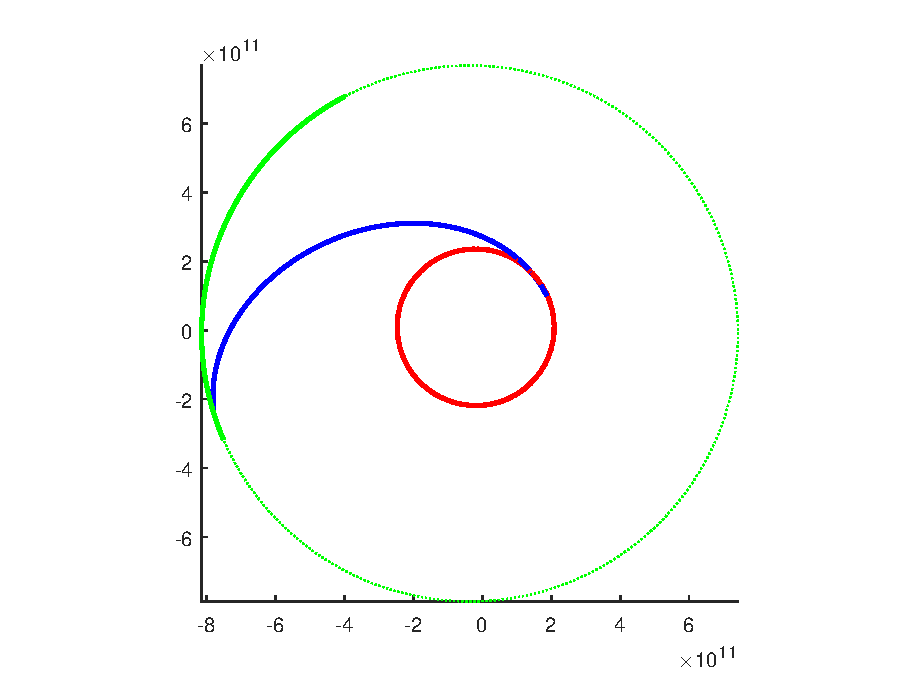
\includegraphics[scale=0.8]{./plots/ex2}
	\caption{Òrbita interplanetària del segon cas resolt}
\end{figure}

\section{Cas de la Terra a Mart}
\begin{itemize}
	\item Sortida: $t_{1}=$2020 Març 06

$\vec{r}_{T}(t_{1})=\begin{bmatrix}-0.9684 & 0.2176 & 0.0000\end{bmatrix}$ AU

	\item Òrbita interplanetària: $\Delta t=95$ dies

$\Delta\lambda=135.697^{\circ}$

$\Delta\theta=135.670^{\circ}$
\begin{table}[h!]
	\centering
	\begin{tabular}{ |c|c|c|c|c|c|}
		\hline
		$a$ & $e$ & $\theta_{1}$ & $\omega$ & $i$ & $\Omega$ \\ \hline
		$71.33848$ AU  & $1.01109$ & $306.690^{\circ}$ & $233.310^{\circ}$ & $2.514^{\circ}$ & $345.607^{\circ}$ \\ \hline
	\end{tabular}
	\caption{Elements orbitals del tercer cas resolt}
\end{table}

	\item Arribada: $t_{2}=$2020 Juny 09

$\vec{r}_{M}(t_{2})=\begin{bmatrix}0.7378 & -1.1916 & -0.0431\end{bmatrix}$ AU
\end{itemize}
\begin{figure}[H]
	\centering
	\includegraphics[scale=0.95]{./plots/ex3}
	\caption{Òrbita interplanetària del tercer cas resolt}
\end{figure}

\section{Cas 1 de Mart a Júpiter}
\begin{itemize}
	\item Sortida: $t_{1}=$2037 Octubre 25

$\vec{r}_{M}(t_{1})=\begin{bmatrix}1.0628 & 0.9973 & -0.0052\end{bmatrix}$ AU

$\vec{v}_{s}(t_{1})=\begin{bmatrix}-21.4616 & 17.6853 & 0.6145\end{bmatrix}$ km/s

$\vec{v}_{\infty_{1}}= \begin{bmatrix}-5.8071 & -2.0496 & -0.1839\end{bmatrix}$ km/s

$\Delta v=4.7546$ km/s

	\item Òrbita interplanetària: $\Delta t=$ dies

$\Delta\lambda=121.960^{\circ}$

$\Delta\theta=121.957^{\circ}$
\begin{table}[h!]
	\centering
	\begin{tabular}{ |c|c|c|c|c|c|}
		\hline
		$a$ & $e$ & $\theta_{1}$ & $\omega$ & $i$ & $\Omega$ \\ \hline
		$3.87684$ AU  & $0.64755$ & $32.516^{\circ}$ & $317.644^{\circ}$ & $1.267^{\circ}$ & $52.502^{\circ}$ \\ \hline
	\end{tabular}
	\caption{Elements orbitals del cas 1}
\end{table}
	\item Arribada: $t_{2}=$2039 Octubre 15

$\vec{r}_{J}(t_{2})=\begin{bmatrix}-5.2121 & 1.4740 & 0.1105\end{bmatrix}$ AU

$\vec{v}_{s}(t_{2})=\begin{bmatrix}-8.6037 & -6.1586 & 0.0680\end{bmatrix}$ km/s


$\vec{v}_{\infty_{2}}=\begin{bmatrix}-4.8918 & 5.8075 & -0.0644\end{bmatrix}$ km/s
\end{itemize}
\begin{figure}[H]
	\centering
	\includegraphics[scale=0.8]{./plots/cas1}
	\caption{Òrbita interplanetària del cas 1}
\end{figure}

\section{Cas 2 de la Terra a Mart}
\begin{itemize}
	\item Sortida: $t_{1}=$2033 Març 13

$\vec{r}_{T}(t_{1})=\begin{bmatrix}-0.9890 & 0.1028 & 0.0000\end{bmatrix}$ AU

$\vec{v}_{s}(t_{1})=\begin{bmatrix}9.9048 & -31.9421 & -1.1405\end{bmatrix}$ km/s

$\vec{v}_{\infty_{1}}= \begin{bmatrix}13.4689 & -2.2007 & -1.1405\end{bmatrix}$ km/s

$\Delta v=9.8291$ km/s

	\item Òrbita interplanetària: $\Delta t=145$ dies

$\Delta\lambda=126.666^{\circ}$

$\Delta\theta=126.647^{\circ}$
\begin{table}[h!]
	\centering
	\begin{tabular}{ |c|c|c|c|c|c|}
		\hline
		$a$ & $e$ & $\theta_{1}$ & $\omega$ & $i$ & $\Omega$ \\ \hline
		$1.34585$ AU  & $0.26502$ & $347.845^{\circ}$ & $192.155^{\circ}$ & $2.154^{\circ}$ & $352.263^{\circ}$ \\ \hline
	\end{tabular}
	\caption{Elements orbitals del cas 2}
\end{table}
	\item Arribada: $t_{2}=$2033 Agost 05

$\vec{r}_{M}(t_{2})=\begin{bmatrix}0.6911 & -1.2225 & -0.0426\end{bmatrix}$ AU

$\vec{v}_{s}(t_{2})=\begin{bmatrix}20.3889 & 10.7059 & 0.5023\end{bmatrix}$ km/s


$\vec{v}_{\infty_{2}}=\begin{bmatrix}-1.6222 & -3.2966 & 0.7500\end{bmatrix}$ km/s
\end{itemize}
\begin{figure}[H]
	\centering
	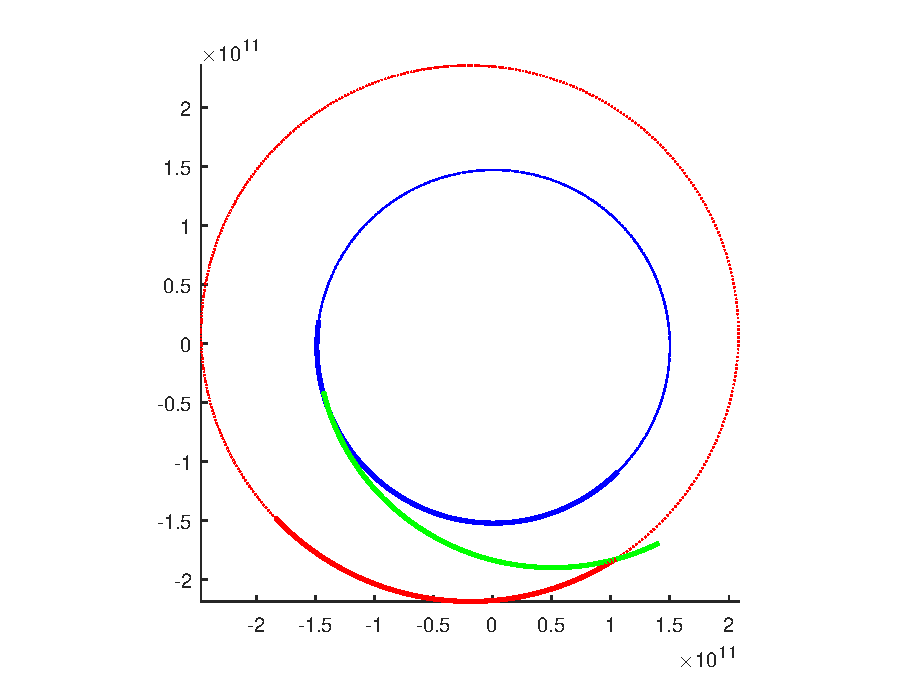
\includegraphics[scale=0.8]{./plots/cas2}
	\caption{Òrbita interplanetària del cas 2}
\end{figure}

\section{Cas 3 de la Terra a Mart}
\begin{itemize}
	\item Sortida: $t_{1}=$2031 Gener 23

$\vec{r}_{T}(t_{1})=\begin{bmatrix}-0.5527 & 0.8145 & 0.0000\end{bmatrix}$ AU

$\vec{v}_{s}(t_{1})=\begin{bmatrix}-27.9432 & -17.5505 & 1.3211\end{bmatrix}$ km/s

$\vec{v}_{\infty_{1}}= \begin{bmatrix}-2.8084 & -0.7119 & 1.3212\end{bmatrix}$ km/s

$\Delta v=3.5559$ km/s

	\item Òrbita interplanetària: $\Delta t=190$ dies

$\Delta\lambda=148.092^{\circ}$

$\Delta\theta=148.071^{\circ}$
\begin{table}[h!]
	\centering
	\begin{tabular}{ |c|c|c|c|c|c|}
		\hline
		$a$ & $e$ & $\theta_{1}$ & $\omega$ & $i$ & $\Omega$ \\ \hline
		$1.24568$ AU  & $0.20996$ & $1.674^{\circ}$ & $358.471^{\circ}$ & $2.293^{\circ}$ & $122.188^{\circ}$ \\ \hline
	\end{tabular}
	\caption{Elements orbitals del cas 3}
\end{table}
	\item Arribada: $t_{2}=$2031 Agost 01

$\vec{r}_{M}(t_{2})=\begin{bmatrix}0.0231 & -1.4528 & -0.0310\end{bmatrix}$ AU

$\vec{v}_{s}(t_{2})=\begin{bmatrix}22.3536 & -2.8628 & -0.6964\end{bmatrix}$ km/s


$\vec{v}_{\infty_{2}}=\begin{bmatrix}-2.7906 & -5.3291 & -0.1299\end{bmatrix}$ km/s
\end{itemize}
\begin{figure}[H]
	\centering
	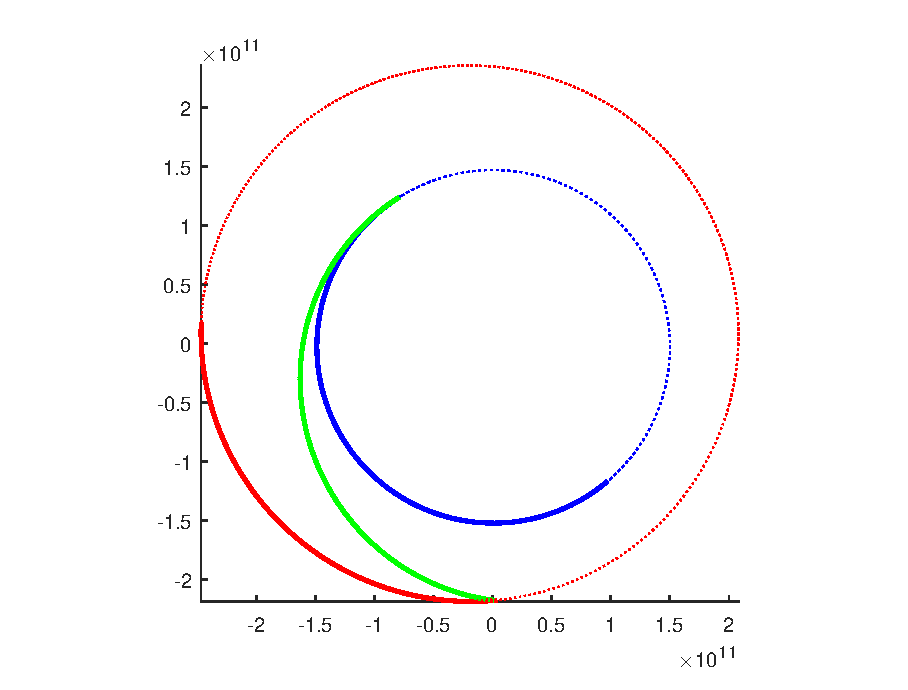
\includegraphics[scale=0.8]{./plots/cas3}
	\caption{Òrbita interplanetària del cas 3}
\end{figure}

\section{Cas 4 de la Terra a Mart}
\begin{itemize}
	\item Sortida: $t_{1}=$2025 Juliol 18

$\vec{r}_{T}(t_{1})=\begin{bmatrix}0.4609 & -0.9057 & 0.0000\end{bmatrix}$ AU

$\vec{v}_{s}(t_{1})=\begin{bmatrix}23.7170 & 8.0146 & -0.2439\end{bmatrix}$ km/s

$\vec{v}_{\infty_{1}}= \begin{bmatrix}5.0303 & 30.9264 & -0.2439\end{bmatrix}$ km/s

$\Delta v=25.6087$ km/s

	\item Òrbita interplanetària: $\Delta t=95$ dies

$\Delta\lambda=308.176^{\circ}$

$\Delta\theta=51.825^{\circ}$

\begin{table}[h!]
	\centering
	\begin{tabular}{ |c|c|c|c|c|c|}
		\hline
		$a$ & $e$ & $\theta_{1}$ & $\omega$ & $i$ & $\Omega$ \\ \hline
		$1.07039$ AU  & $0.46551$ & $112.076^{\circ}$ & $67.350^{\circ}$ & $0.563^{\circ}$ & $115.868^{\circ}$ \\ \hline
	\end{tabular}
	\caption{Elements orbitals del cas 4}
\end{table}
	\item Arribada: $t_{2}=$2025 Octubre 21

$\vec{r}_{M}(t_{2})=\begin{bmatrix}-0.6676 & -1.3608 & -0.0121\end{bmatrix}$ AU

$\vec{v}_{s}(t_{2})=\begin{bmatrix}2.1862 & 17.3824 & -0.0938\end{bmatrix}$ km/s


$\vec{v}_{\infty_{2}}=\begin{bmatrix}-20.4827 & 25.9781 & 0.6436\end{bmatrix}$ km/s
\end{itemize}
\pagebreak

\section{Cas 5 de la Terra a Venus}
\begin{itemize}
	\item Sortida: $t_{1}=$2023 Maig 27

$\vec{r}_{T}(t_{1})=\begin{bmatrix}-0.3986 & -0.9317 & 0.0000\end{bmatrix}$ AU

$\vec{v}_{s}(t_{1})=\begin{bmatrix}23.5396 & -11.9653 & -0.7732\end{bmatrix}$ km/s

$\vec{v}_{\infty_{1}}= \begin{bmatrix}-3.3635 & -0.1365 & -0.7731\end{bmatrix}$ km/s

$\Delta v=3.6369$ km/s

	\item Òrbita interplanetària: $\Delta t=158$ dies

$\Delta\lambda=202.000^{\circ}$

$\Delta\theta=157.992^{\circ}$
\begin{table}[h!]
	\centering
	\begin{tabular}{ |c|c|c|c|c|c|}
		\hline
		$a$ & $e$ & $\theta_{1}$ & $\omega$ & $i$ & $\Omega$ \\ \hline
		$0.86221$ AU  & $0.23212$ & $147.050^{\circ}$ & $32.950^{\circ}$ & $1.678^{\circ}$ & $65.165^{\circ}$ \\ \hline
	\end{tabular}
	\caption{Elements orbitals del cas 5}
\end{table}

	\item Arribada: $t_{2}=$2023 Novembre 01

$\vec{r}_{V}(t_{2})=\begin{bmatrix}0.0215 & 0.7194 & 0.0086\end{bmatrix}$ AU

$\vec{v}_{s}(t_{2})=\begin{bmatrix}-34.9238 & 17.3219 & 1.1418\end{bmatrix}$ km/s


$\vec{v}_{\infty_{2}}=\begin{bmatrix}0.2017 & 16.4570 & -0.8976\end{bmatrix}$ km/s
\end{itemize}
\begin{figure}[H]
	\centering
	\includegraphics[scale=0.8]{./plots/cas5}
	\caption{Òrbita interplanetària del cas 5}
\end{figure}

\section{Cas 6 de Mart a la Terra}
\begin{itemize}
	\item Sortida: $t_{1}=$2033 Gener 18

$\vec{r}_{M}(t_{1})=\begin{bmatrix}-1.5798 & -0.4008 & 0.0304\end{bmatrix}$ AU

$\vec{v}_{s}(t_{1})=\begin{bmatrix}-3.4918 & -19.9512 & 0.5779\end{bmatrix}$ km/s

$\vec{v}_{\infty_{1}}= \begin{bmatrix}-10.3564 & 1.4666 & 1.1954\end{bmatrix}$ km/s

$\Delta v=7.4443$ km/s

	\item Òrbita interplanetària: $\Delta t=222$ dies

$\Delta\lambda=140.675^{\circ}$

$\Delta\theta=140.663^{\circ}$
\begin{table}[h!]
	\centering
	\begin{tabular}{ |c|c|c|c|c|c|}
		\hline
		$a$ & $e$ & $\theta_{1}$ & $\omega$ & $i$ & $\Omega$ \\ \hline
		$1.31415$ AU  & $0.24918$ & $191.345^{\circ}$ & $207.993^{\circ}$ & $1.696^{\circ}$ & $154.559^{\circ}$ \\ \hline
	\end{tabular}
	\caption{Elements orbitals del cas 6}
\end{table}

	\item Arribada: $t_{2}=$2033 Agost 28

$\vec{r}_{T}(t_{2})=\begin{bmatrix}0.9246 & -0.4059 & 0.0000\end{bmatrix}$ AU

$\vec{v}_{s}(t_{2})=\begin{bmatrix}25.3126 & 14.6475 & -0.7136\end{bmatrix}$ km/s


$\vec{v}_{\infty_{2}}=\begin{bmatrix}13.8240 & -12.5180 & -0.7137\end{bmatrix}$ km/s
\end{itemize}
\begin{figure}[H]
	\centering
	\includegraphics[scale=0.8]{./plots/cas6}
	\caption{Òrbita interplanetària del cas 6}
\end{figure}

\section{Cas 7 de Mart a la Terra}
\begin{itemize}
	\item Sortida: $t_{1}=$2030 Novembre 20

$\vec{r}_{M}(t_{1})=\begin{bmatrix}-1.4214 & 0.8647 & 0.0531\end{bmatrix}$ AU

$\vec{v}_{s}(t_{1})=\begin{bmatrix}-13.0320 & -14.8691 & 0.7226\end{bmatrix}$ km/s

$\vec{v}_{\infty_{1}}= \begin{bmatrix}-1.3512 & 3.7651 & 0.8259\end{bmatrix}$ km/s

$\Delta v=3.8493$ km/s

	\item Òrbita interplanetària: $\Delta t=228$ dies

$\Delta\lambda=134.956^{\circ}$

$\Delta\theta=134.927^{\circ}$
\begin{table}[h!]
	\centering
	\begin{tabular}{ |c|c|c|c|c|c|}
		\hline
		$a$ & $e$ & $\theta_{1}$ & $\omega$ & $i$ & $\Omega$ \\ \hline
		$1.31613$ AU  & $0.26617$ & $184.700^{\circ}$ & $220.499^{\circ}$ & $2.572^{\circ}$ & $103.210^{\circ}$ \\ \hline
	\end{tabular}
	\caption{Elements orbitals del cas 7}
\end{table}
	\item Arribada: $t_{2}=$2031 Juliol 06

$\vec{r}_{T}(t_{2})=\begin{bmatrix}0.2640 & -0.9818 & 0.0000\end{bmatrix}$ AU

$\vec{v}_{s}(t_{2})=\begin{bmatrix}30.9612 & 26.0696 & -1.3808\end{bmatrix}$ km/s


$\vec{v}_{\infty_{2}}=\begin{bmatrix}2.6783 & -5.0153 & -1.3808\end{bmatrix}$ km/s
\end{itemize}
\begin{figure}[H]
	\centering
	\includegraphics[scale=0.8]{./plots/cas7}
	\caption{Òrbita interplanetària del cas 7}
\end{figure}

\section{Cas 8 de la Terra a Mart}
\begin{itemize}
	\item Sortida: $t_{1}=$2021 Novembre 26

$\vec{r}_{T}(t_{1})=\begin{bmatrix}0.4106 & 0.8971 & 0.0000\end{bmatrix}$ AU

	\item Òrbita interplanetària: $\Delta t=85$ dies

$\Delta\lambda=198.239^{\circ}$

$\Delta\theta=161.735^{\circ}$
\begin{table}[h!]
	\centering
	\begin{tabular}{ |c|c|c|c|c|c|}
		\hline
		$a$ & $e$ & $\theta_{1}$ & $\omega$ & $i$ & $\Omega$ \\ \hline
		$1.34032$ AU  & $1.44253$ & $288.926^{\circ}$ & $251.074^{\circ}$ & $3.166^{\circ}$ & $243.635^{\circ}$ \\ \hline
	\end{tabular}
	\caption{Elements orbitals del cas 8}
\end{table}

	\item Arribada: $t_{2}=$2022 Febrer 19

$\vec{r}_{M}(t_{2})=\begin{bmatrix}-0.1973 & -1.4584 & -0.0257\end{bmatrix}$ AU
\end{itemize}
\begin{figure}[H]
	\centering
	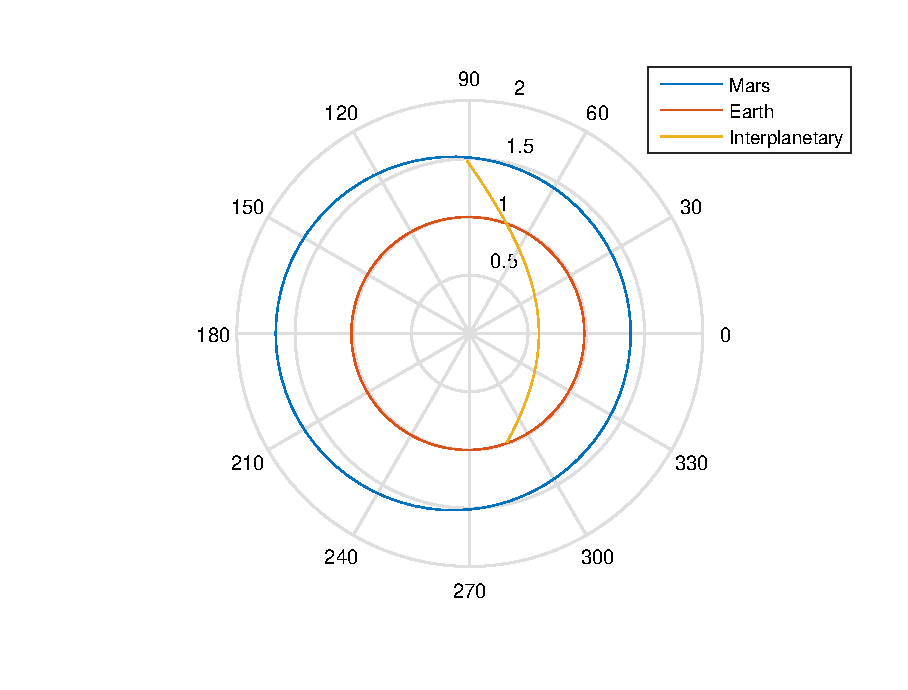
\includegraphics[scale=0.95]{./plots/cas8}
	\caption{Òrbita interplanetària del cas 8}
\end{figure}

\section{Cas 9 de la Terra a Mart}
\begin{itemize}
	\item Sortida: $t_{1}=$2022 Gener 15

$\vec{r}_{T}(t_{1})=\begin{bmatrix}-0.4355 & 0.8821 & 0.0000\end{bmatrix}$ AU

	\item Òrbita interplanetària: $\Delta t=95$ dies

$\Delta\lambda=182.508^{\circ}$

$\Delta\theta=176.966^{\circ}$
\begin{table}[h!]
	\centering
	\begin{tabular}{ |c|c|c|c|c|c|}
		\hline
		$a$ & $e$ & $\theta_{1}$ & $\omega$ & $i$ & $\Omega$ \\ \hline
		$5.10048$ AU  & $1.11071$ & $280.991^{\circ}$ & $259.009^{\circ}$ & $34.288^{\circ}$ & $294.501^{\circ}$ \\ \hline
	\end{tabular}
	\caption{Elements orbitals del cas 9}
\end{table}

	\item Arribada: $t_{2}=$2022 Abril 20

$\vec{r}_{M}(t_{2})=\begin{bmatrix}0.6495 & -1.2481 & -0.0421\end{bmatrix}$ AU
\end{itemize}
\begin{figure}[H]
	\centering
	\includegraphics[scale=0.95]{./plots/cas9}
	\caption{Òrbita interplanetària del cas 9}
\end{figure}